\documentclass{article}

% Language setting
% Replace `english' with e.g. `spanish' to change the document language
\usepackage[english]{babel}
\usepackage[font=small,labelfont=bf]{caption}
% Set page size and margins
% Replace `letterpaper' with `a4paper' for UK/EU standard size
\usepackage[letterpaper,top=2cm,bottom=2cm,left=3cm,right=3cm,marginparwidth=1.75cm]{geometry}

% Useful packages
\usepackage{amsmath}
\usepackage{graphicx}
\usepackage[colorlinks=true, allcolors=blue]{hyperref}

\title{Analyzing the Impact of Overlapping Clustering on the Large Scale Citation Networks}
\author{A Jakatdar, T Warnow, G Chacko}

\begin{document}
\maketitle

\begin{abstract}
Community detection has become an important task in bibliometrics, where the collection of publications connected by citations into citation networks has become the primary medium by which this task has been solved through. A variety of methods have been proposed in detecting such communities, with a focus on clustering algorithms, but there has yet to be an effort to utilize overlapping clustering methods to detect communities within these citation networks. This paper proposes a scalable, overlapping clustering method designed to detect communities, and compares this method to an existing disjoint clustering method proposed in Wedell et al. 
\end{abstract}

\section{Introduction}
\section{Related Works}
\subsection{KMP Pipeline: Wedell et al}




\subsection{Overlapping Clustering Method: Evans \& Lambiotte}

\subsection{Tier Analysis: Chandrasekaran et al}

\subsection{Breadth/Depth \& Independence/Dependence: Bu et al}


\section{Dataset}

In order to compare our proposed overlapping method with the disjoint KMP-valid clustering method proposed in Wedell et al, we can test our method on the same SABPQ expansion Exosome Citation Network with two modifications from the original dataset used in Wedell et al in order to remove any information in our network that may be counterintuitive for the task of community detection. 

\subsection{Retracted Papers}

[Add George's Work Here]

\subsection{High Referencing Papers}

\section{Overlapping KMP Pipeline Method}

We can now defined a proposed method to solve the overlapping clustering problem of community detection using a pipeline similar to the one used to create KMP-valid clusterings in Wedell et al. 

\subsection{Input}
The inputs to this method are a clustering file and a network file, where the clustering file represents a valid clustering of the network in the network file. The clustering file should be a tab separated values (tsv) clustering file with two columns, the first column representing the cluster index and the second column representing the publication index of a publication in the corresponding cluster. The network file should be a tsv network file with two columns, the first column representing the source node index and the second column representing the sink node index.
\newline\newline
We can formally define the input pipeline run to generate the clustering file using a modified version of the Wedell et al. KMP-valid pipeline as shown below.
\newline\newline
\begin{center}
    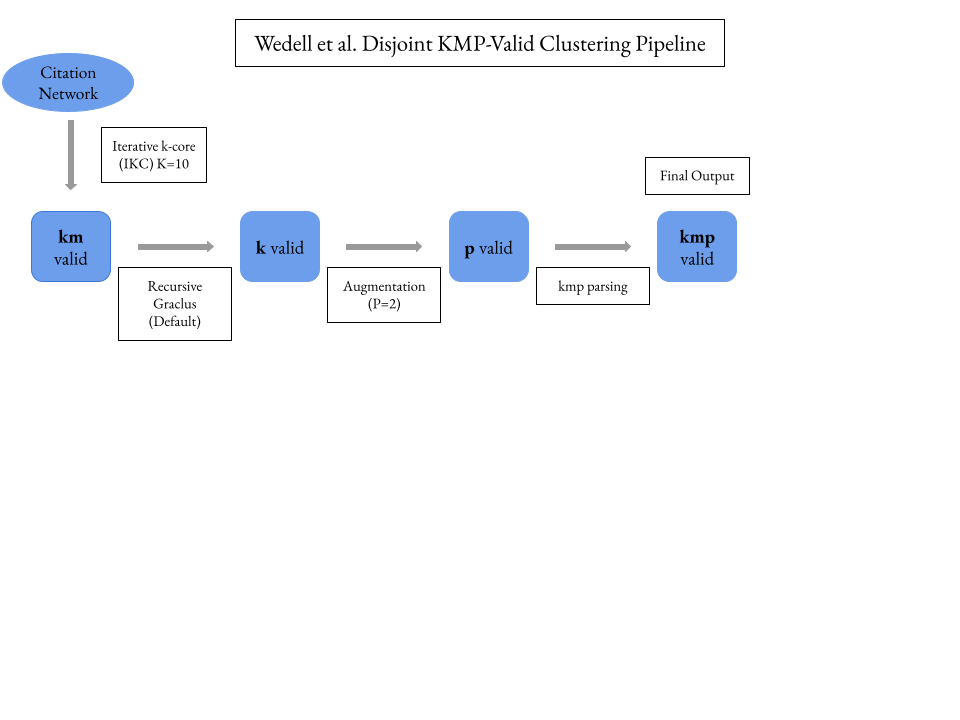
\includegraphics[trim={0 12cm 0 0},clip, scale=0.5]{Overlapping Pipeline Drawing.png}
    \captionof{figure}{The input disjoint KMP-valid clustering pipeline for k=10, p=2 using the default Recursive Graclus and the default kmp-parsing. Step 2 and Step 3 of hte pipeline remain unchanged for all input clusterings observed in this paper. }
\end{center}
\newline\newline
We can define two such constraint problems that our overlapping clustering method aims to utilizing in both the candidate selection step and cluster inclusion step. Both such constraint problems are described below. 

\subsection{Candidate Selection Step}
We can begin by defining the constraint problem that we are trying to satisfy when deciding which publications to select as candidate publications. In dealing with large networks with $>1$ million nodes, the candidate selection step is necessary to narrow the search space for the cluster inclusion step. Instead of dealing with the entire network, we can deal with a focused subspace based on some cost function and constraints, in order to generate an easier-to-process candidate set for the cluster inclusion stage.
\newline\newline
We define a valid candidate selection constraint inequality to have the form $c(n, N) \leq T$ for some cost function $c$ and threshold value $T$ for a node $n \in N$. The cost function takes as input any node $n$ from the network $N$ and computes a heuristic cost score to predict its fit in multiple clusters. By minimizing the cost function with respect to a threshold, we select not just the best singular candidate, but a set of candidates that satisfy the inequality. 
\newline\newline
The cost function we decide to use for the contents of this paper is the rank of the total degree of a publication (citations + references), with a threshold $T=10000$. In layman terms, we select the top $10000$ publications ranked by total degree as our candidate selection criteria. Formally put, our cost function can be described as follows:
$$\text{degree}(n) = \text{citations(n)} + \text{references(n)}$$
$$c(n', N) = \text{rank}(\text{degree}(n'), \{\text{degree}(n) | \forall n \in N\}) \leq 10000$$
All publications that satisfy this inequality in the network will be added to a candidate set to be processed in the cluster inclusion step. 
\subsection{Cluster Inclusion Step}
We can now define the constraint problem that we are trying to satisfy when deciding whether or not to include a candidate publication in a cluster outside of its original disjoint cluster. While the candidate selection step involves a cost function that we are trying to minimize with respect to a certain threshold, the cluster inclusion step involves maximizing a score function $s$ with respect to a certain threshold $T$ with the form $s(n, C) \geq T$ for some input disjoint clustering $C$.
\newline\newline
The scoring function we decided to use for the contents of this paper is the total number of adjacent core publications found in the cluster, and the threshold value $T$ that we will consider for experiments in this paper is the Minimum Core Degree (MCD) of the cluster to be considered for inclusion. In layman terms, in order for a candidate publication to be included in a cluster, it must be adjacent to at least the T neighbors in the cluster such that $T \geq MCD$ so that the MCD of the cluster is conserved. Formully put, our scoring function can be described as follows:
$$s(n, C) =\sum_{n' \in C} A[n][n'] \geq MCD(C)$$
All candidate publications that satisfy this inequality for any given cluster will be added to that respective cluster. 



\section{Experiments}

We can now design experiments to understand certain core components of our overlapping clustering method compared to disjoint clustering methods like KMP-valid clustering. Firstly, comparing out overlapping clustering method across different candidate selection criteria and cluster inclusion criteria for both node coveragem edge coverage and cluster size metrics can be seen below. 
\begin{center}
    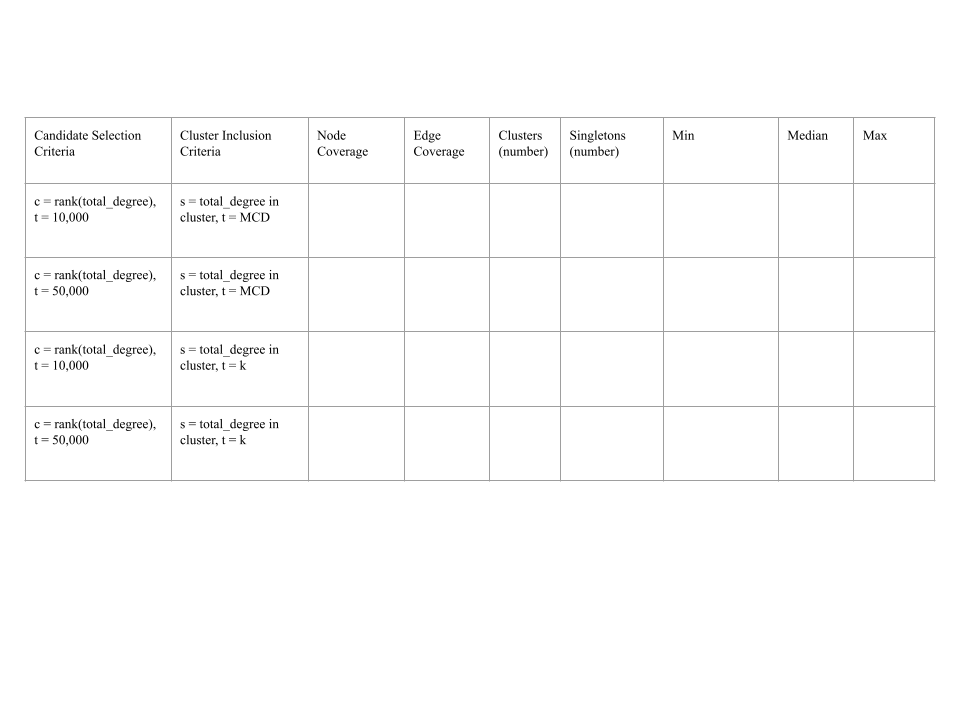
\includegraphics[trim={0 7cm 0 3cm},clip, scale=0.5]{Overlapping Clusters Tables.png}
    \captionof{figure}{}
\end{center}
\newline\newline

Once we notice which specific criteria give the best node coverage and edge coverage, we can compare the top two to 

\end{document}